\documentclass[]{article}
\usepackage{lmodern}
\usepackage{amssymb,amsmath}
\usepackage{ifxetex,ifluatex}
\usepackage{fixltx2e} % provides \textsubscript
\ifnum 0\ifxetex 1\fi\ifluatex 1\fi=0 % if pdftex
  \usepackage[T1]{fontenc}
  \usepackage[utf8]{inputenc}
\else % if luatex or xelatex
  \ifxetex
    \usepackage{mathspec}
    \usepackage{xltxtra,xunicode}
  \else
    \usepackage{fontspec}
  \fi
  \defaultfontfeatures{Mapping=tex-text,Scale=MatchLowercase}
  \newcommand{\euro}{€}
\fi
% use upquote if available, for straight quotes in verbatim environments
\IfFileExists{upquote.sty}{\usepackage{upquote}}{}
% use microtype if available
\IfFileExists{microtype.sty}{%
\usepackage{microtype}
\UseMicrotypeSet[protrusion]{basicmath} % disable protrusion for tt fonts
}{}
\usepackage[margin=1in]{geometry}
\ifxetex
  \usepackage[setpagesize=false, % page size defined by xetex
              unicode=false, % unicode breaks when used with xetex
              xetex]{hyperref}
\else
  \usepackage[unicode=true]{hyperref}
\fi
\hypersetup{breaklinks=true,
            bookmarks=true,
            pdfauthor={},
            pdftitle={},
            colorlinks=true,
            citecolor=blue,
            urlcolor=blue,
            linkcolor=magenta,
            pdfborder={0 0 0}}
\urlstyle{same}  % don't use monospace font for urls
\usepackage{color}
\usepackage{fancyvrb}
\newcommand{\VerbBar}{|}
\newcommand{\VERB}{\Verb[commandchars=\\\{\}]}
\DefineVerbatimEnvironment{Highlighting}{Verbatim}{commandchars=\\\{\}}
% Add ',fontsize=\small' for more characters per line
\usepackage{framed}
\definecolor{shadecolor}{RGB}{248,248,248}
\newenvironment{Shaded}{\begin{snugshade}}{\end{snugshade}}
\newcommand{\KeywordTok}[1]{\textcolor[rgb]{0.13,0.29,0.53}{\textbf{{#1}}}}
\newcommand{\DataTypeTok}[1]{\textcolor[rgb]{0.13,0.29,0.53}{{#1}}}
\newcommand{\DecValTok}[1]{\textcolor[rgb]{0.00,0.00,0.81}{{#1}}}
\newcommand{\BaseNTok}[1]{\textcolor[rgb]{0.00,0.00,0.81}{{#1}}}
\newcommand{\FloatTok}[1]{\textcolor[rgb]{0.00,0.00,0.81}{{#1}}}
\newcommand{\ConstantTok}[1]{\textcolor[rgb]{0.00,0.00,0.00}{{#1}}}
\newcommand{\CharTok}[1]{\textcolor[rgb]{0.31,0.60,0.02}{{#1}}}
\newcommand{\SpecialCharTok}[1]{\textcolor[rgb]{0.00,0.00,0.00}{{#1}}}
\newcommand{\StringTok}[1]{\textcolor[rgb]{0.31,0.60,0.02}{{#1}}}
\newcommand{\VerbatimStringTok}[1]{\textcolor[rgb]{0.31,0.60,0.02}{{#1}}}
\newcommand{\SpecialStringTok}[1]{\textcolor[rgb]{0.31,0.60,0.02}{{#1}}}
\newcommand{\ImportTok}[1]{{#1}}
\newcommand{\CommentTok}[1]{\textcolor[rgb]{0.56,0.35,0.01}{\textit{{#1}}}}
\newcommand{\DocumentationTok}[1]{\textcolor[rgb]{0.56,0.35,0.01}{\textbf{\textit{{#1}}}}}
\newcommand{\AnnotationTok}[1]{\textcolor[rgb]{0.56,0.35,0.01}{\textbf{\textit{{#1}}}}}
\newcommand{\CommentVarTok}[1]{\textcolor[rgb]{0.56,0.35,0.01}{\textbf{\textit{{#1}}}}}
\newcommand{\OtherTok}[1]{\textcolor[rgb]{0.56,0.35,0.01}{{#1}}}
\newcommand{\FunctionTok}[1]{\textcolor[rgb]{0.00,0.00,0.00}{{#1}}}
\newcommand{\VariableTok}[1]{\textcolor[rgb]{0.00,0.00,0.00}{{#1}}}
\newcommand{\ControlFlowTok}[1]{\textcolor[rgb]{0.13,0.29,0.53}{\textbf{{#1}}}}
\newcommand{\OperatorTok}[1]{\textcolor[rgb]{0.81,0.36,0.00}{\textbf{{#1}}}}
\newcommand{\BuiltInTok}[1]{{#1}}
\newcommand{\ExtensionTok}[1]{{#1}}
\newcommand{\PreprocessorTok}[1]{\textcolor[rgb]{0.56,0.35,0.01}{\textit{{#1}}}}
\newcommand{\AttributeTok}[1]{\textcolor[rgb]{0.77,0.63,0.00}{{#1}}}
\newcommand{\RegionMarkerTok}[1]{{#1}}
\newcommand{\InformationTok}[1]{\textcolor[rgb]{0.56,0.35,0.01}{\textbf{\textit{{#1}}}}}
\newcommand{\WarningTok}[1]{\textcolor[rgb]{0.56,0.35,0.01}{\textbf{\textit{{#1}}}}}
\newcommand{\AlertTok}[1]{\textcolor[rgb]{0.94,0.16,0.16}{{#1}}}
\newcommand{\ErrorTok}[1]{\textcolor[rgb]{0.64,0.00,0.00}{\textbf{{#1}}}}
\newcommand{\NormalTok}[1]{{#1}}
\usepackage{longtable,booktabs}
\usepackage{graphicx,grffile}
\makeatletter
\def\maxwidth{\ifdim\Gin@nat@width>\linewidth\linewidth\else\Gin@nat@width\fi}
\def\maxheight{\ifdim\Gin@nat@height>\textheight\textheight\else\Gin@nat@height\fi}
\makeatother
% Scale images if necessary, so that they will not overflow the page
% margins by default, and it is still possible to overwrite the defaults
% using explicit options in \includegraphics[width, height, ...]{}
\setkeys{Gin}{width=\maxwidth,height=\maxheight,keepaspectratio}
\setlength{\parindent}{0pt}
\setlength{\parskip}{6pt plus 2pt minus 1pt}
\setlength{\emergencystretch}{3em}  % prevent overfull lines
\providecommand{\tightlist}{%
  \setlength{\itemsep}{0pt}\setlength{\parskip}{0pt}}
\setcounter{secnumdepth}{0}

%%% Use protect on footnotes to avoid problems with footnotes in titles
\let\rmarkdownfootnote\footnote%
\def\footnote{\protect\rmarkdownfootnote}

%%% Change title format to be more compact
\usepackage{titling}

% Create subtitle command for use in maketitle
\newcommand{\subtitle}[1]{
  \posttitle{
    \begin{center}\large#1\end{center}
    }
}

\setlength{\droptitle}{-2em}
  \title{}
  \pretitle{\vspace{\droptitle}}
  \posttitle{}
  \author{}
  \preauthor{}\postauthor{}
  \date{}
  \predate{}\postdate{}


% Redefines (sub)paragraphs to behave more like sections
\ifx\paragraph\undefined\else
\let\oldparagraph\paragraph
\renewcommand{\paragraph}[1]{\oldparagraph{#1}\mbox{}}
\fi
\ifx\subparagraph\undefined\else
\let\oldsubparagraph\subparagraph
\renewcommand{\subparagraph}[1]{\oldsubparagraph{#1}\mbox{}}
\fi

\begin{document}
\maketitle

\section{Stuff You Should Know About: Handling Large Data Files with
R}\label{stuff-you-should-know-about-handling-large-data-files-with-r}

\subsection{The Data Table package and various other ways to handle data
in
R}\label{the-data-table-package-and-various-other-ways-to-handle-data-in-r}

\begin{itemize}
\tightlist
\item
  \textbf{Authors}: Tom Kelly
\item
  \textbf{Research field}: Bioinformatics / Computational Biology /
  Cancer Genomics
\item
  \textbf{Lesson Topic}: An introduction to various packages for file
  I/O and data manipulation in R, with comparision to base R (and
  compatibility with data frames), in terms of user-friendliness,
  performance in CPU-time, and memory usage.
\end{itemize}

\subsection{Installation}\label{installation}

Install Data Table from CRAN (current version 1.9.6)

\begin{Shaded}
\begin{Highlighting}[]
\KeywordTok{install.packages}\NormalTok{(}\StringTok{"data.table"}\NormalTok{, }\DataTypeTok{repos =} \StringTok{"https::/cran.rstudio.com"}\NormalTok{)}
\KeywordTok{library}\NormalTok{(}\StringTok{"data.table"}\NormalTok{)}
\end{Highlighting}
\end{Shaded}

Install development version from GitHub (current version 1.9.7)

\begin{Shaded}
\begin{Highlighting}[]
\KeywordTok{install.packages}\NormalTok{(}\StringTok{"data.table"}\NormalTok{, }\DataTypeTok{repos =} \StringTok{"https://Rdatatable.github.io/data.table"}\NormalTok{, }\DataTypeTok{type =} \StringTok{"source"}\NormalTok{) }\CommentTok{#v1.9.7}
\KeywordTok{library}\NormalTok{(}\StringTok{"data.table"}\NormalTok{)}
\end{Highlighting}
\end{Shaded}

\subsection{Getting Started: Data
Frames}\label{getting-started-data-frames}

data table has it's own read function - to rapidly read data into R
Backwards compatible: It can be used for data.frames

\begin{Shaded}
\begin{Highlighting}[]
\NormalTok{gapminderFiveYearData <-}\StringTok{ }\KeywordTok{fread}\NormalTok{(}\StringTok{"gapminder-FiveYearData.csv"}\NormalTok{, }\DataTypeTok{data.table=}\NormalTok{F)}
\KeywordTok{class}\NormalTok{(gapminderFiveYearData)}
\end{Highlighting}
\end{Shaded}

\begin{verbatim}
## [1] "data.frame"
\end{verbatim}

\begin{Shaded}
\begin{Highlighting}[]
\KeywordTok{dim}\NormalTok{(gapminderFiveYearData)}
\end{Highlighting}
\end{Shaded}

\begin{verbatim}
## [1] 1704    6
\end{verbatim}

\begin{Shaded}
\begin{Highlighting}[]
\KeywordTok{head}\NormalTok{(gapminderFiveYearData)}
\end{Highlighting}
\end{Shaded}

\begin{verbatim}
##       country year      pop continent lifeExp gdpPercap
## 1 Afghanistan 1952  8425333      Asia  28.801  779.4453
## 2 Afghanistan 1957  9240934      Asia  30.332  820.8530
## 3 Afghanistan 1962 10267083      Asia  31.997  853.1007
## 4 Afghanistan 1967 11537966      Asia  34.020  836.1971
## 5 Afghanistan 1972 13079460      Asia  36.088  739.9811
## 6 Afghanistan 1977 14880372      Asia  38.438  786.1134
\end{verbatim}

\begin{Shaded}
\begin{Highlighting}[]
\KeywordTok{tail}\NormalTok{(gapminderFiveYearData)}
\end{Highlighting}
\end{Shaded}

\begin{verbatim}
##       country year      pop continent lifeExp gdpPercap
## 1699 Zimbabwe 1982  7636524    Africa  60.363  788.8550
## 1700 Zimbabwe 1987  9216418    Africa  62.351  706.1573
## 1701 Zimbabwe 1992 10704340    Africa  60.377  693.4208
## 1702 Zimbabwe 1997 11404948    Africa  46.809  792.4500
## 1703 Zimbabwe 2002 11926563    Africa  39.989  672.0386
## 1704 Zimbabwe 2007 12311143    Africa  43.487  469.7093
\end{verbatim}

\begin{Shaded}
\begin{Highlighting}[]
\KeywordTok{str}\NormalTok{(gapminderFiveYearData)}
\end{Highlighting}
\end{Shaded}

\begin{verbatim}
## 'data.frame':    1704 obs. of  6 variables:
##  $ country  : chr  "Afghanistan" "Afghanistan" "Afghanistan" "Afghanistan" ...
##  $ year     : int  1952 1957 1962 1967 1972 1977 1982 1987 1992 1997 ...
##  $ pop      : num  8425333 9240934 10267083 11537966 13079460 ...
##  $ continent: chr  "Asia" "Asia" "Asia" "Asia" ...
##  $ lifeExp  : num  28.8 30.3 32 34 36.1 ...
##  $ gdpPercap: num  779 821 853 836 740 ...
\end{verbatim}

Backwards compatible: these are standard dataframes compatible with
ggplots

\begin{Shaded}
\begin{Highlighting}[]
\KeywordTok{library}\NormalTok{(}\StringTok{"ggplot2"}\NormalTok{)}
\KeywordTok{ggplot}\NormalTok{(}\DataTypeTok{data =} \NormalTok{gapminderFiveYearData, }\KeywordTok{aes}\NormalTok{(}\DataTypeTok{x =} \NormalTok{lifeExp, }\DataTypeTok{y =} \NormalTok{gdpPercap, }\DataTypeTok{color=}\NormalTok{continent)) +}
\StringTok{  }\KeywordTok{geom_point}\NormalTok{()}
\end{Highlighting}
\end{Shaded}

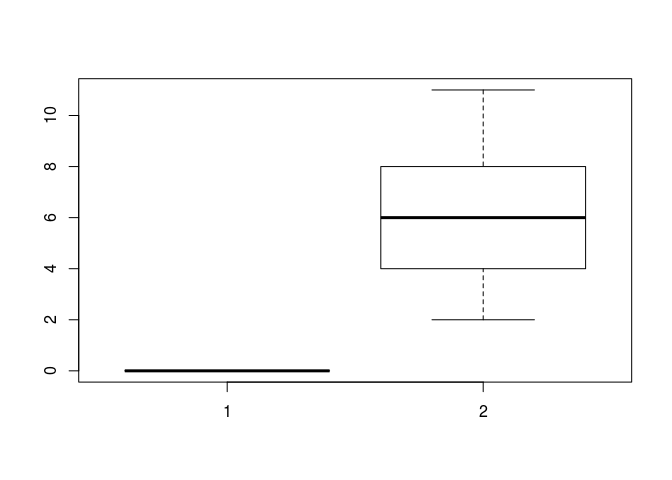
\includegraphics{Figs/unnamed-chunk-4-1.pdf}\\
 \#\#Introducing Data Tables

data table defaults to reading it's own data.table format

\begin{Shaded}
\begin{Highlighting}[]
\NormalTok{gapminderFiveYearData <-}\StringTok{ }\KeywordTok{fread}\NormalTok{(}\StringTok{"gapminder-FiveYearData.csv"}\NormalTok{)}
\KeywordTok{class}\NormalTok{(gapminderFiveYearData)}
\end{Highlighting}
\end{Shaded}

\begin{verbatim}
## [1] "data.table" "data.frame"
\end{verbatim}

\begin{Shaded}
\begin{Highlighting}[]
\KeywordTok{dim}\NormalTok{(gapminderFiveYearData)}
\end{Highlighting}
\end{Shaded}

\begin{verbatim}
## [1] 1704    6
\end{verbatim}

\begin{Shaded}
\begin{Highlighting}[]
\KeywordTok{head}\NormalTok{(gapminderFiveYearData)}
\end{Highlighting}
\end{Shaded}

\begin{verbatim}
##        country year      pop continent lifeExp gdpPercap
## 1: Afghanistan 1952  8425333      Asia  28.801  779.4453
## 2: Afghanistan 1957  9240934      Asia  30.332  820.8530
## 3: Afghanistan 1962 10267083      Asia  31.997  853.1007
## 4: Afghanistan 1967 11537966      Asia  34.020  836.1971
## 5: Afghanistan 1972 13079460      Asia  36.088  739.9811
## 6: Afghanistan 1977 14880372      Asia  38.438  786.1134
\end{verbatim}

\begin{Shaded}
\begin{Highlighting}[]
\KeywordTok{tail}\NormalTok{(gapminderFiveYearData)}
\end{Highlighting}
\end{Shaded}

\begin{verbatim}
##     country year      pop continent lifeExp gdpPercap
## 1: Zimbabwe 1982  7636524    Africa  60.363  788.8550
## 2: Zimbabwe 1987  9216418    Africa  62.351  706.1573
## 3: Zimbabwe 1992 10704340    Africa  60.377  693.4208
## 4: Zimbabwe 1997 11404948    Africa  46.809  792.4500
## 5: Zimbabwe 2002 11926563    Africa  39.989  672.0386
## 6: Zimbabwe 2007 12311143    Africa  43.487  469.7093
\end{verbatim}

\begin{Shaded}
\begin{Highlighting}[]
\KeywordTok{str}\NormalTok{(gapminderFiveYearData)}
\end{Highlighting}
\end{Shaded}

\begin{verbatim}
## Classes 'data.table' and 'data.frame':   1704 obs. of  6 variables:
##  $ country  : chr  "Afghanistan" "Afghanistan" "Afghanistan" "Afghanistan" ...
##  $ year     : int  1952 1957 1962 1967 1972 1977 1982 1987 1992 1997 ...
##  $ pop      : num  8425333 9240934 10267083 11537966 13079460 ...
##  $ continent: chr  "Asia" "Asia" "Asia" "Asia" ...
##  $ lifeExp  : num  28.8 30.3 32 34 36.1 ...
##  $ gdpPercap: num  779 821 853 836 740 ...
##  - attr(*, ".internal.selfref")=<externalptr>
\end{verbatim}

Data tables also auto-trim when printing to console

\begin{Shaded}
\begin{Highlighting}[]
\NormalTok{gapminderFiveYearData}
\end{Highlighting}
\end{Shaded}

\begin{verbatim}
##           country year      pop continent lifeExp gdpPercap
##    1: Afghanistan 1952  8425333      Asia  28.801  779.4453
##    2: Afghanistan 1957  9240934      Asia  30.332  820.8530
##    3: Afghanistan 1962 10267083      Asia  31.997  853.1007
##    4: Afghanistan 1967 11537966      Asia  34.020  836.1971
##    5: Afghanistan 1972 13079460      Asia  36.088  739.9811
##   ---                                                      
## 1700:    Zimbabwe 1987  9216418    Africa  62.351  706.1573
## 1701:    Zimbabwe 1992 10704340    Africa  60.377  693.4208
## 1702:    Zimbabwe 1997 11404948    Africa  46.809  792.4500
## 1703:    Zimbabwe 2002 11926563    Africa  39.989  672.0386
## 1704:    Zimbabwe 2007 12311143    Africa  43.487  469.7093
\end{verbatim}

data tables are backwards compatible with a lot of operations which use
data.frames Such as plots\ldots{}

\begin{Shaded}
\begin{Highlighting}[]
\KeywordTok{ggplot}\NormalTok{(}\DataTypeTok{data =} \NormalTok{gapminderFiveYearData, }\KeywordTok{aes}\NormalTok{(}\DataTypeTok{x =} \NormalTok{lifeExp, }\DataTypeTok{y =} \NormalTok{gdpPercap, }\DataTypeTok{color=}\NormalTok{continent)) +}
\StringTok{  }\KeywordTok{geom_point}\NormalTok{()}
\end{Highlighting}
\end{Shaded}

\includegraphics{Figs/unnamed-chunk-7-1.pdf}\\
\ldots{} and linear models\ldots{}

\begin{Shaded}
\begin{Highlighting}[]
\NormalTok{linear_model <-}\StringTok{ }\KeywordTok{lm}\NormalTok{(gdpPercap ~}\StringTok{ }\NormalTok{pop +}\StringTok{ }\NormalTok{year, gapminderFiveYearData)}
\KeywordTok{summary}\NormalTok{(linear_model)}
\end{Highlighting}
\end{Shaded}

\begin{verbatim}
## 
## Call:
## lm(formula = gdpPercap ~ pop + year, data = gapminderFiveYearData)
## 
## Residuals:
##    Min     1Q Median     3Q    Max 
## -10537  -5356  -2811   2043 109153 
## 
## Coefficients:
##               Estimate Std. Error t value Pr(>|t|)    
## (Intercept) -2.537e+05  2.674e+04  -9.487   <2e-16 ***
## pop         -4.143e-06  2.198e-06  -1.885   0.0596 .  
## year         1.319e+02  1.351e+01   9.760   <2e-16 ***
## ---
## Signif. codes:  0 '***' 0.001 '**' 0.01 '*' 0.05 '.' 0.1 ' ' 1
## 
## Residual standard error: 9595 on 1701 degrees of freedom
## Multiple R-squared:  0.05365,    Adjusted R-squared:  0.05254 
## F-statistic: 48.22 on 2 and 1701 DF,  p-value: < 2.2e-16
\end{verbatim}

\begin{Shaded}
\begin{Highlighting}[]
\NormalTok{linear_model <-}\StringTok{ }\KeywordTok{lm}\NormalTok{(lifeExp ~}\StringTok{ }\NormalTok{gdpPercap +}\StringTok{ }\NormalTok{pop +}\StringTok{ }\NormalTok{year, gapminderFiveYearData)}
\KeywordTok{summary}\NormalTok{(linear_model)}
\end{Highlighting}
\end{Shaded}

\begin{verbatim}
## 
## Call:
## lm(formula = lifeExp ~ gdpPercap + pop + year, data = gapminderFiveYearData)
## 
## Residuals:
##     Min      1Q  Median      3Q     Max 
## -67.497  -7.075   1.121   7.701  19.640 
## 
## Coefficients:
##               Estimate Std. Error t value Pr(>|t|)    
## (Intercept) -4.115e+02  2.767e+01 -14.872  < 2e-16 ***
## gdpPercap    6.729e-04  2.444e-05  27.529  < 2e-16 ***
## pop          6.353e-09  2.218e-09   2.864  0.00423 ** 
## year         2.354e-01  1.400e-02  16.812  < 2e-16 ***
## ---
## Signif. codes:  0 '***' 0.001 '**' 0.01 '*' 0.05 '.' 0.1 ' ' 1
## 
## Residual standard error: 9.673 on 1700 degrees of freedom
## Multiple R-squared:  0.4402, Adjusted R-squared:  0.4392 
## F-statistic: 445.6 on 3 and 1700 DF,  p-value: < 2.2e-16
\end{verbatim}

\begin{Shaded}
\begin{Highlighting}[]
\NormalTok{linear_model <-}\StringTok{ }\KeywordTok{glm}\NormalTok{(lifeExp ~}\StringTok{ }\NormalTok{gdpPercap +}\StringTok{ }\NormalTok{continent +}\StringTok{ }\NormalTok{pop +}\StringTok{ }\NormalTok{year, }\DataTypeTok{family  =}\StringTok{"gaussian"}\NormalTok{, gapminderFiveYearData)}
\KeywordTok{summary}\NormalTok{(linear_model)}
\end{Highlighting}
\end{Shaded}

\begin{verbatim}
## 
## Call:
## glm(formula = lifeExp ~ gdpPercap + continent + pop + year, family = "gaussian", 
##     data = gapminderFiveYearData)
## 
## Deviance Residuals: 
##      Min        1Q    Median        3Q       Max  
## -28.4051   -4.0550    0.2317    4.5073   20.0217  
## 
## Coefficients:
##                     Estimate Std. Error t value Pr(>|t|)    
## (Intercept)       -5.185e+02  1.989e+01 -26.062   <2e-16 ***
## gdpPercap          2.985e-04  2.002e-05  14.908   <2e-16 ***
## continentAmericas  1.429e+01  4.946e-01  28.898   <2e-16 ***
## continentAsia      9.375e+00  4.719e-01  19.869   <2e-16 ***
## continentEurope    1.936e+01  5.182e-01  37.361   <2e-16 ***
## continentOceania   2.056e+01  1.469e+00  13.995   <2e-16 ***
## pop                1.791e-09  1.634e-09   1.096    0.273    
## year               2.863e-01  1.006e-02  28.469   <2e-16 ***
## ---
## Signif. codes:  0 '***' 0.001 '**' 0.01 '*' 0.05 '.' 0.1 ' ' 1
## 
## (Dispersion parameter for gaussian family taken to be 47.37935)
## 
##     Null deviance: 284148  on 1703  degrees of freedom
## Residual deviance:  80355  on 1696  degrees of freedom
## AIC: 11420
## 
## Number of Fisher Scoring iterations: 2
\end{verbatim}

\ldots{} and data manipulation packages (plyr, dplyr, reshape, tidyr,
etc\ldots{})

\begin{Shaded}
\begin{Highlighting}[]
\KeywordTok{library}\NormalTok{(}\StringTok{"plyr"}\NormalTok{)}
\NormalTok{calcGDP <-}\StringTok{ }\NormalTok{function(dat, }\DataTypeTok{year=}\OtherTok{NULL}\NormalTok{, }\DataTypeTok{country=}\OtherTok{NULL}\NormalTok{) \{}
  \NormalTok{if(!}\KeywordTok{is.null}\NormalTok{(year)) \{}
    \NormalTok{dat <-}\StringTok{ }\NormalTok{dat[dat$year %in%}\StringTok{ }\NormalTok{year, ]}
  \NormalTok{\}}
  \NormalTok{if (!}\KeywordTok{is.null}\NormalTok{(country)) \{}
    \NormalTok{dat <-}\StringTok{ }\NormalTok{dat[dat$country %in%}\StringTok{ }\NormalTok{country,]}
  \NormalTok{\}}
  \NormalTok{gdp <-}\StringTok{ }\NormalTok{dat$pop *}\StringTok{ }\NormalTok{dat$gdpPercap}
  
  \NormalTok{new <-}\StringTok{ }\KeywordTok{cbind}\NormalTok{(dat, }\DataTypeTok{gdp=}\NormalTok{gdp)}
  \KeywordTok{return}\NormalTok{(new)}
\NormalTok{\}}
\NormalTok{plyr::}\KeywordTok{ddply}\NormalTok{(}
  \DataTypeTok{.data =} \KeywordTok{calcGDP}\NormalTok{(gapminderFiveYearData),}
  \DataTypeTok{.variables =} \StringTok{"continent"}\NormalTok{,}
  \DataTypeTok{.fun =} \NormalTok{function(x) }\KeywordTok{mean}\NormalTok{(x$gdp)}
\NormalTok{)}
\end{Highlighting}
\end{Shaded}

\begin{verbatim}
##   continent           V1
## 1    Africa  20904782844
## 2  Americas 379262350210
## 3      Asia 227233738153
## 4    Europe 269442085301
## 5   Oceania 188187105354
\end{verbatim}

Yeah you get the idea.

Data tables have built-in ``methods'' for a range of functions, these
are often faster than standard dataframes or matrices, if these aren't
found it uses dataframe functions. A ``Data Table'' is compatible with
any function from any package designed for a ``Data Frame''.

\subsection{File I/O (Input/Output)}\label{file-io-inputoutput}

fread is ``fast read'', and it's \textbf{fast}, even for large data
files. Let's try it out on some larger datafiles:

\begin{Shaded}
\begin{Highlighting}[]
\NormalTok{gapminderlarge <-}\StringTok{ }\KeywordTok{fread}\NormalTok{(}\StringTok{"gapminder-large.csv"}\NormalTok{, }\DataTypeTok{header=}\NormalTok{T)}
\end{Highlighting}
\end{Shaded}

fread is smart, it auto detects column classes, separators, headers,
nrows (for a regularly separated file). We can use the same comand for a
whole bunch of file formats. All the usual reading options can be
specified manually\ldots{}

\begin{Shaded}
\begin{Highlighting}[]
\NormalTok{gapminderFiveYearData <-}\StringTok{ }\KeywordTok{fread}\NormalTok{(}\StringTok{"gapminder-FiveYearData.tsv"}\NormalTok{) }\CommentTok{#tab delimited}
\NormalTok{gapminderFiveYearData <-}\StringTok{ }\KeywordTok{fread}\NormalTok{(}\StringTok{"gapminder-FiveYearData.txt"}\NormalTok{) }\CommentTok{#space delimited}
\NormalTok{gapminderFiveYearDataCrop <-}\StringTok{ }\KeywordTok{fread}\NormalTok{(}\StringTok{"gapminder-FiveYearData.tsv"}\NormalTok{, }\DataTypeTok{header=}\NormalTok{T, }\DataTypeTok{col.names=}\KeywordTok{c}\NormalTok{(}\StringTok{"place"}\NormalTok{, }\StringTok{"time"}\NormalTok{, }\StringTok{"people"}\NormalTok{, }\StringTok{"big place"}\NormalTok{, }\StringTok{"life"}\NormalTok{, }\StringTok{"money"}\NormalTok{), }\DataTypeTok{nrows=}\DecValTok{1000}\NormalTok{, }\DataTypeTok{stringsAsFactors=}\NormalTok{F)}
\NormalTok{gapminderFiveYearDataCrop}
\end{Highlighting}
\end{Shaded}

\begin{verbatim}
##             place time    people big place   life      money
##    1: Afghanistan 1952   8425333      Asia 28.801   779.4453
##    2: Afghanistan 1957   9240934      Asia 30.332   820.8530
##    3: Afghanistan 1962  10267083      Asia 31.997   853.1007
##    4: Afghanistan 1967  11537966      Asia 34.020   836.1971
##    5: Afghanistan 1972  13079460      Asia 36.088   739.9811
##   ---                                                       
##  996:      Mexico 2007 108700891  Americas 76.195 11977.5750
##  997:    Mongolia 1952    800663      Asia 42.244   786.5669
##  998:    Mongolia 1957    882134      Asia 45.248   912.6626
##  999:    Mongolia 1962   1010280      Asia 48.251  1056.3540
## 1000:    Mongolia 1967   1149500      Asia 51.253  1226.0411
\end{verbatim}

\ldots{}but it does a lot of the tedious work for you (pretty well too).

It's also got cool progress bars for large files :) These kick in
automatically if the file takes longer than about a second. This is
really handy to know your code is working, and how long it will take.

\begin{Shaded}
\begin{Highlighting}[]
\NormalTok{gapminderlarger <-}\StringTok{ }\KeywordTok{fread}\NormalTok{(}\StringTok{"gapminder-larger.csv"}\NormalTok{)}
\end{Highlighting}
\end{Shaded}

\begin{verbatim}
## 
Read 42.7% of 6625152 rows
Read 71.2% of 6625152 rows
Read 99.5% of 6625152 rows
Read 6625152 rows and 6 (of 6) columns from 0.321 GB file in 00:00:05
\end{verbatim}

It's so fast it tells you. Let's compare that with base R:

\begin{Shaded}
\begin{Highlighting}[]
\KeywordTok{system.time}\NormalTok{(gapminderlarger.dataframe <-}\StringTok{ }\KeywordTok{read.csv}\NormalTok{(}\StringTok{"gapminder-larger.csv"}\NormalTok{, }\DataTypeTok{header=}\NormalTok{T))}
\end{Highlighting}
\end{Shaded}

\begin{verbatim}
##    user  system elapsed 
##  22.128   0.288  22.440
\end{verbatim}

The same operation took much longer with base R, with larger files (or
repeating this many times) that \textasciitilde{}6x difference could
mean a lot for your workflow.

FYI - there's also a ``fast write'' compatible with several file formats

\begin{Shaded}
\begin{Highlighting}[]
\KeywordTok{fwrite}\NormalTok{(gapminderlarger, }\DataTypeTok{file=}\StringTok{"test.csv"}\NormalTok{) }\CommentTok{#defaults to csv}
\KeywordTok{fwrite}\NormalTok{(gapminderlarger, }\DataTypeTok{file=}\StringTok{"test.tsv"}\NormalTok{, }\DataTypeTok{sep=}\StringTok{"}\CharTok{\textbackslash{}t}\StringTok{"}\NormalTok{)}
\end{Highlighting}
\end{Shaded}

They're also fast to write data, compared to base R:

\begin{Shaded}
\begin{Highlighting}[]
\KeywordTok{system.time}\NormalTok{(}\KeywordTok{fwrite}\NormalTok{(gapminderlarger, }\DataTypeTok{file=}\StringTok{"test.csv"}\NormalTok{))}
\end{Highlighting}
\end{Shaded}

\begin{verbatim}
##    user  system elapsed 
##  17.616   0.440  19.775
\end{verbatim}

\begin{Shaded}
\begin{Highlighting}[]
\KeywordTok{system.time}\NormalTok{(}\KeywordTok{write.csv}\NormalTok{(gapminderlarger, }\DataTypeTok{file=}\StringTok{"test.csv"}\NormalTok{))}
\end{Highlighting}
\end{Shaded}

\begin{verbatim}
##    user  system elapsed 
##  39.484   0.396  42.705
\end{verbatim}

\subsection{readr (Hadley Wickham and
RStudio)}\label{readr-hadley-wickham-and-rstudio}

Another package enables faster alternatives to existing read functions
in base R: these work almost exactly the same as their base R
counterparts.

\begin{longtable}[c]{@{}lll@{}}
\toprule
\textbf{base R} & \textbf{readr}\tabularnewline
\midrule
\endhead
spaced file & \texttt{read.table} & \texttt{read\_table}\tabularnewline
fixed-width file & \texttt{read.fwf} & \texttt{read\_fwf}\tabularnewline
comma-separated file & \texttt{read.csv} &
\texttt{read\_csv}\tabularnewline
semicolon-separated file & \texttt{read.csv2} &
\texttt{read\_csv2}\tabularnewline
tab-delimited file & \texttt{read.table} &
\texttt{read\_tsv}\tabularnewline
comma-separated file & \texttt{read.csv} &
\texttt{read\_csv}\tabularnewline
file or string \texttt{readLines} & \texttt{read\_lines} or
\texttt{read\_file}\tabularnewline
\bottomrule
\end{longtable}

Let's try it out on a space-delimited file:

\begin{Shaded}
\begin{Highlighting}[]
\KeywordTok{library}\NormalTok{(}\StringTok{"readr"}\NormalTok{)}
\KeywordTok{system.time}\NormalTok{(}\KeywordTok{read_table}\NormalTok{(}\StringTok{"gapminder-FiveYearData.txt"}\NormalTok{))}
\end{Highlighting}
\end{Shaded}

\begin{verbatim}
##    user  system elapsed 
##   0.024   0.000   0.022
\end{verbatim}

\begin{Shaded}
\begin{Highlighting}[]
\KeywordTok{system.time}\NormalTok{(}\KeywordTok{read.table}\NormalTok{(}\StringTok{"gapminder-FiveYearData.txt"}\NormalTok{))}
\end{Highlighting}
\end{Shaded}

\begin{verbatim}
##    user  system elapsed 
##   0.012   0.000   0.012
\end{verbatim}

Even on a small file \texttt{readr} is faster than base R. This also
holds for larger csv files:

\begin{Shaded}
\begin{Highlighting}[]
\KeywordTok{system.time}\NormalTok{(}\KeywordTok{read_csv}\NormalTok{(}\StringTok{"gapminder-larger.csv"}\NormalTok{))}
\end{Highlighting}
\end{Shaded}

\begin{verbatim}
##    user  system elapsed 
##   4.452   0.040   4.499
\end{verbatim}

\begin{Shaded}
\begin{Highlighting}[]
\KeywordTok{system.time}\NormalTok{(}\KeywordTok{read.csv}\NormalTok{(}\StringTok{"gapminder-larger.csv"}\NormalTok{))}
\end{Highlighting}
\end{Shaded}

\begin{verbatim}
##    user  system elapsed 
##  21.960   0.348  22.333
\end{verbatim}

\texttt{readr} also has a handy progress bar allowign us to monitor
progress. There is an equivalent \texttt{readxl} package with a
\texttt{read\_excel} function compatible with xls or xlsx files and
enables sheet selection. This is a relatively new alternative to the
\texttt{xlsx} package and it's \texttt{read.xlsx} function which are
difficult to work with (as it is java and perl dependent).

\subsection{Another solution:
bigmemory}\label{another-solution-bigmemory}

\begin{Shaded}
\begin{Highlighting}[]
\KeywordTok{library}\NormalTok{(}\StringTok{"bigmemory"}\NormalTok{)}
\end{Highlighting}
\end{Shaded}

``bigmemory'' uses the ``big.matrix'' format to access large data files
in a C++ framework - rather than stored in RAM/memory as usual in R.
This is handy for handling \textbf{very large} files, when loading the
full dataset in working environment (RAM memory) slows your computer to
a halt. Might be handy on servers / HPC too but usually they have enough
memory if you're willing to wait for it in a queue.

Let's try out bigmemory, first we convert an R data matrix into a
``big.matrix'':

\begin{Shaded}
\begin{Highlighting}[]
\NormalTok{gapminderFiveYearData.big <-}\StringTok{ }\KeywordTok{as.big.matrix}\NormalTok{(gapminderFiveYearData)}
\NormalTok{gapminderFiveYearData.big}
\end{Highlighting}
\end{Shaded}

\begin{verbatim}
## An object of class "big.matrix"
## Slot "address":
## <pointer: 0x9455710>
\end{verbatim}

\begin{Shaded}
\begin{Highlighting}[]
\KeywordTok{class}\NormalTok{(gapminderFiveYearData.big)}
\end{Highlighting}
\end{Shaded}

\begin{verbatim}
## [1] "big.matrix"
## attr(,"package")
## [1] "bigmemory"
\end{verbatim}

\begin{Shaded}
\begin{Highlighting}[]
\KeywordTok{dim}\NormalTok{(gapminderFiveYearData.big)}
\end{Highlighting}
\end{Shaded}

\begin{verbatim}
## [1] 1704    6
\end{verbatim}

\begin{Shaded}
\begin{Highlighting}[]
\KeywordTok{head}\NormalTok{(gapminderFiveYearData.big)}
\end{Highlighting}
\end{Shaded}

\begin{verbatim}
##   country year      pop continent lifeExp gdpPercap
## 1       1 1952  8425333         3  28.801  779.4453
## 2       1 1957  9240934         3  30.332  820.8530
## 3       1 1962 10267083         3  31.997  853.1007
## 4       1 1967 11537966         3  34.020  836.1971
## 5       1 1972 13079460         3  36.088  739.9811
## 6       1 1977 14880372         3  38.438  786.1134
\end{verbatim}

\begin{Shaded}
\begin{Highlighting}[]
\KeywordTok{tail}\NormalTok{(gapminderFiveYearData.big)}
\end{Highlighting}
\end{Shaded}

\begin{verbatim}
##      country year      pop continent lifeExp gdpPercap
## 1699     142 1982  7636524         1  60.363  788.8550
## 1700     142 1987  9216418         1  62.351  706.1573
## 1701     142 1992 10704340         1  60.377  693.4208
## 1702     142 1997 11404948         1  46.809  792.4500
## 1703     142 2002 11926563         1  39.989  672.0386
## 1704     142 2007 12311143         1  43.487  469.7093
\end{verbatim}

\begin{Shaded}
\begin{Highlighting}[]
\KeywordTok{str}\NormalTok{(gapminderFiveYearData.big)}
\end{Highlighting}
\end{Shaded}

\begin{verbatim}
## Formal class 'big.matrix' [package "bigmemory"] with 1 slot
##   ..@ address:<externalptr>
\end{verbatim}

bigmemory, also has read/write functions direct to big.matrix format:

\begin{Shaded}
\begin{Highlighting}[]
\KeywordTok{write.big.matrix}\NormalTok{(gapminderFiveYearData.big, }\StringTok{"test.csv"}\NormalTok{)}
\NormalTok{gapminderFiveYearData.big <-}\StringTok{ }\KeywordTok{read.big.matrix}\NormalTok{(}\StringTok{"test.csv"}\NormalTok{)}
\end{Highlighting}
\end{Shaded}

These are designed to be efficient for memory - how fast are they?

\begin{Shaded}
\begin{Highlighting}[]
\KeywordTok{system.time}\NormalTok{(gapminderlarger.big <-}\StringTok{ }\KeywordTok{read.big.matrix}\NormalTok{(}\StringTok{"gapminder-larger.csv"}\NormalTok{))}
\end{Highlighting}
\end{Shaded}

\begin{verbatim}
##    user  system elapsed 
##  12.680   0.188  12.883
\end{verbatim}

\begin{Shaded}
\begin{Highlighting}[]
\KeywordTok{system.time}\NormalTok{(}\KeywordTok{write.big.matrix}\NormalTok{(gapminderFiveYearData.big, }\StringTok{"test.csv"}\NormalTok{))}
\end{Highlighting}
\end{Shaded}

\begin{verbatim}
##    user  system elapsed 
##   0.012   0.000   0.012
\end{verbatim}

\subsection{New and Shiny: FEATHER}\label{new-and-shiny-feather}

\subsubsection{A Fast On-Disk Format for Data Frames for R and Python,
powered by Apache
Arrow}\label{a-fast-on-disk-format-for-data-frames-for-r-and-python-powered-by-apache-arrow}

FEATHER (is it's own fast file format) - from Hadley Wickham
ggplot/dplyr/etc\ldots{} and Wes Mckinney (pandas in Python) Note: it's
in development (unstable) - future versions may not read past versions -
intended for use to transfer files quickly (e.g., between R and Python)

At the moment you can only try it out from their github repo (in R or
python), it will no doubt end up on CRAN very soon:

\begin{Shaded}
\begin{Highlighting}[]
\KeywordTok{library}\NormalTok{(}\StringTok{"devtools"}\NormalTok{)}
\NormalTok{devtools::}\KeywordTok{install_github}\NormalTok{(}\StringTok{"wesm/feather/R"}\NormalTok{)}
\KeywordTok{library}\NormalTok{(feather)}
\end{Highlighting}
\end{Shaded}

FEATHER has it's own file I/O commands (and format):

\begin{Shaded}
\begin{Highlighting}[]
\NormalTok{path <-}\StringTok{ "gapminder-FiveYearData.feather"}
\KeywordTok{write_feather}\NormalTok{(gapminderFiveYearData, path) }\CommentTok{#write data frame to file}
\NormalTok{gapminderFiveYearData <-}\StringTok{ }\KeywordTok{read_feather}\NormalTok{(path) }\CommentTok{#read to data frame}
\NormalTok{gapminderFiveYearData}
\end{Highlighting}
\end{Shaded}

\begin{verbatim}
## Source: local data frame [1,704 x 6]
## 
##        country  year      pop continent lifeExp gdpPercap
##          <chr> <int>    <dbl>     <chr>   <dbl>     <dbl>
## 1  Afghanistan  1952  8425333      Asia  28.801  779.4453
## 2  Afghanistan  1957  9240934      Asia  30.332  820.8530
## 3  Afghanistan  1962 10267083      Asia  31.997  853.1007
## 4  Afghanistan  1967 11537966      Asia  34.020  836.1971
## 5  Afghanistan  1972 13079460      Asia  36.088  739.9811
## 6  Afghanistan  1977 14880372      Asia  38.438  786.1134
## 7  Afghanistan  1982 12881816      Asia  39.854  978.0114
## 8  Afghanistan  1987 13867957      Asia  40.822  852.3959
## 9  Afghanistan  1992 16317921      Asia  41.674  649.3414
## 10 Afghanistan  1997 22227415      Asia  41.763  635.3414
## ..         ...   ...      ...       ...     ...       ...
\end{verbatim}

Did I mention it's crazy fast?

\begin{Shaded}
\begin{Highlighting}[]
\NormalTok{path <-}\StringTok{ "gapminderlarger.feather"}
\KeywordTok{system.time}\NormalTok{(}\KeywordTok{write_feather}\NormalTok{(gapminderlarger, path))}
\end{Highlighting}
\end{Shaded}

\begin{verbatim}
##    user  system elapsed 
##   0.304   0.224   1.570
\end{verbatim}

\begin{Shaded}
\begin{Highlighting}[]
\KeywordTok{system.time}\NormalTok{(gapminderlarger.feather <-}\StringTok{ }\KeywordTok{read_feather}\NormalTok{(path))}
\end{Highlighting}
\end{Shaded}

\begin{verbatim}
##    user  system elapsed 
##   0.332   0.024   0.358
\end{verbatim}

Or install and run in Python:

\begin{verbatim}
import feather
path = 'my_data.feather'
feather.write_dataframe(df, path)
df = feather.read_dataframe(path)
\end{verbatim}

Note that FEATHER is designed for data \emph{already} loaded into python
or R.

\subsection{FILE I/O Summary}\label{file-io-summary}

\subsubsection{READ}\label{read}

\begin{longtable}[c]{@{}lllll@{}}
\toprule
\begin{minipage}[b]{0.05\columnwidth}\raggedright\strut
\textbf{base R}
\strut\end{minipage} &
\begin{minipage}[b]{0.05\columnwidth}\raggedright\strut
\textbf{data table}
\strut\end{minipage} &
\begin{minipage}[b]{0.05\columnwidth}\raggedright\strut
\textbf{readr}
\strut\end{minipage} &
\begin{minipage}[b]{0.05\columnwidth}\raggedright\strut
\textbf{bigmemory}
\strut\end{minipage} &
\begin{minipage}[b]{0.05\columnwidth}\raggedright\strut
\textbf{feather}
\strut\end{minipage}\tabularnewline
\midrule
\endhead
\begin{minipage}[t]{0.05\columnwidth}\raggedright\strut
\texttt{read.csv}
\strut\end{minipage} &
\begin{minipage}[t]{0.05\columnwidth}\raggedright\strut
\texttt{fread}
\strut\end{minipage} &
\begin{minipage}[t]{0.05\columnwidth}\raggedright\strut
\texttt{read\_csv}
\strut\end{minipage} &
\begin{minipage}[t]{0.05\columnwidth}\raggedright\strut
\texttt{read.big.matrix}
\strut\end{minipage} &
\begin{minipage}[t]{0.05\columnwidth}\raggedright\strut
\texttt{read\_feather}
\strut\end{minipage}\tabularnewline
\begin{minipage}[t]{0.05\columnwidth}\raggedright\strut
52.203s
\strut\end{minipage} &
\begin{minipage}[t]{0.05\columnwidth}\raggedright\strut
8.154s
\strut\end{minipage} &
\begin{minipage}[t]{0.05\columnwidth}\raggedright\strut
11.120s
\strut\end{minipage} &
\begin{minipage}[t]{0.05\columnwidth}\raggedright\strut
28.647s
\strut\end{minipage} &
\begin{minipage}[t]{0.05\columnwidth}\raggedright\strut
2.414s
\strut\end{minipage}\tabularnewline
\bottomrule
\end{longtable}

\subsubsection{Convert dataframe to
format}\label{convert-dataframe-to-format}

\begin{longtable}[c]{@{}llll@{}}
\toprule
\textbf{base R} & \textbf{data table} & \textbf{bigmemory} &
\textbf{feather}\tabularnewline
\midrule
\endhead
\texttt{data.frame} & \texttt{as.data.table} & \texttt{as.big.matrix} &
built-in\tabularnewline
NA & 0.002s & 66.07s & NA\tabularnewline
\bottomrule
\end{longtable}

\subsubsection{Write}\label{write}

\begin{longtable}[c]{@{}llll@{}}
\toprule
\textbf{base R} & \textbf{data table} & \textbf{bigmemory} &
\textbf{feather}\tabularnewline
\midrule
\endhead
\texttt{write.csv} & \texttt{fwrite} & \texttt{write.big.matrix} &
\texttt{write\_feather}\tabularnewline
71.382s & 35.453s & 0.068ss & 5.008s\tabularnewline
\bottomrule
\end{longtable}

\subsection{Manipulating Data Tables}\label{manipulating-data-tables}

\begin{Shaded}
\begin{Highlighting}[]
\NormalTok{gapminderFiveYearData <-}\StringTok{ }\KeywordTok{fread}\NormalTok{(}\StringTok{"gapminder-FiveYearData.csv"}\NormalTok{, }\DataTypeTok{data.table=}\NormalTok{T, }\DataTypeTok{header =} \NormalTok{T)}
\KeywordTok{class}\NormalTok{(gapminderFiveYearData)}
\end{Highlighting}
\end{Shaded}

\begin{verbatim}
## [1] "data.table" "data.frame"
\end{verbatim}

We can simply treat it as a data frame in many cases:

\begin{Shaded}
\begin{Highlighting}[]
\NormalTok{gapminderFiveYearData[}\DecValTok{1}\NormalTok{,]}
\end{Highlighting}
\end{Shaded}

\begin{verbatim}
##        country year     pop continent lifeExp gdpPercap
## 1: Afghanistan 1952 8425333      Asia  28.801  779.4453
\end{verbatim}

\begin{Shaded}
\begin{Highlighting}[]
\KeywordTok{colnames}\NormalTok{(gapminderFiveYearData)}
\end{Highlighting}
\end{Shaded}

\begin{verbatim}
## [1] "country"   "year"      "pop"       "continent" "lifeExp"   "gdpPercap"
\end{verbatim}

\begin{Shaded}
\begin{Highlighting}[]
\KeywordTok{head}\NormalTok{(gapminderFiveYearData$country)}
\end{Highlighting}
\end{Shaded}

\begin{verbatim}
## [1] "Afghanistan" "Afghanistan" "Afghanistan" "Afghanistan" "Afghanistan"
## [6] "Afghanistan"
\end{verbatim}

\begin{Shaded}
\begin{Highlighting}[]
\KeywordTok{tail}\NormalTok{(gapminderFiveYearData$country)}
\end{Highlighting}
\end{Shaded}

\begin{verbatim}
## [1] "Zimbabwe" "Zimbabwe" "Zimbabwe" "Zimbabwe" "Zimbabwe" "Zimbabwe"
\end{verbatim}

Data Table has a ``Natural'' Syntax

\texttt{DT{[}where,\ select\textbar{}update\textbar{}do,\ by{]}}

\ldots{}although suspiciously similar to SQL?

it allows chaining queries: \texttt{DT{[}{]}{[}{]}}

Formally: we subset a datatable, Dt, with \texttt{DT{[}i,\ j,\ by{]}}

\subsubsection{I: row selection}\label{i-row-selection}

\begin{Shaded}
\begin{Highlighting}[]
\NormalTok{gapminderFiveYearData[}\KeywordTok{c}\NormalTok{(}\DecValTok{1}\NormalTok{:}\DecValTok{5}\NormalTok{, }\DecValTok{100}\NormalTok{:}\DecValTok{105}\NormalTok{),] }\CommentTok{#by number}
\end{Highlighting}
\end{Shaded}

\begin{verbatim}
##         country year       pop continent lifeExp gdpPercap
##  1: Afghanistan 1952   8425333      Asia  28.801  779.4453
##  2: Afghanistan 1957   9240934      Asia  30.332  820.8530
##  3: Afghanistan 1962  10267083      Asia  31.997  853.1007
##  4: Afghanistan 1967  11537966      Asia  34.020  836.1971
##  5: Afghanistan 1972  13079460      Asia  36.088  739.9811
##  6:  Bangladesh 1967  62821884      Asia  43.453  721.1861
##  7:  Bangladesh 1972  70759295      Asia  45.252  630.2336
##  8:  Bangladesh 1977  80428306      Asia  46.923  659.8772
##  9:  Bangladesh 1982  93074406      Asia  50.009  676.9819
## 10:  Bangladesh 1987 103764241      Asia  52.819  751.9794
## 11:  Bangladesh 1992 113704579      Asia  56.018  837.8102
\end{verbatim}

\begin{Shaded}
\begin{Highlighting}[]
\NormalTok{gapminderFiveYearData[gapminderFiveYearData$country==}\StringTok{"New Zealand"}\NormalTok{,] }\CommentTok{#by condition}
\end{Highlighting}
\end{Shaded}

\begin{verbatim}
##         country year     pop continent lifeExp gdpPercap
##  1: New Zealand 1952 1994794   Oceania  69.390  10556.58
##  2: New Zealand 1957 2229407   Oceania  70.260  12247.40
##  3: New Zealand 1962 2488550   Oceania  71.240  13175.68
##  4: New Zealand 1967 2728150   Oceania  71.520  14463.92
##  5: New Zealand 1972 2929100   Oceania  71.890  16046.04
##  6: New Zealand 1977 3164900   Oceania  72.220  16233.72
##  7: New Zealand 1982 3210650   Oceania  73.840  17632.41
##  8: New Zealand 1987 3317166   Oceania  74.320  19007.19
##  9: New Zealand 1992 3437674   Oceania  76.330  18363.32
## 10: New Zealand 1997 3676187   Oceania  77.550  21050.41
## 11: New Zealand 2002 3908037   Oceania  79.110  23189.80
## 12: New Zealand 2007 4115771   Oceania  80.204  25185.01
\end{verbatim}

\begin{Shaded}
\begin{Highlighting}[]
\NormalTok{gapminderFiveYearData[gapminderFiveYearData$country %in%}\StringTok{ }\KeywordTok{c}\NormalTok{(}\StringTok{"New Zealand"}\NormalTok{, }\StringTok{"Australia"}\NormalTok{, }\StringTok{"Japan"}\NormalTok{),] }\CommentTok{#by condition}
\end{Highlighting}
\end{Shaded}

\begin{verbatim}
##         country year       pop continent lifeExp gdpPercap
##  1:   Australia 1952   8691212   Oceania  69.120 10039.596
##  2:   Australia 1957   9712569   Oceania  70.330 10949.650
##  3:   Australia 1962  10794968   Oceania  70.930 12217.227
##  4:   Australia 1967  11872264   Oceania  71.100 14526.125
##  5:   Australia 1972  13177000   Oceania  71.930 16788.629
##  6:   Australia 1977  14074100   Oceania  73.490 18334.198
##  7:   Australia 1982  15184200   Oceania  74.740 19477.009
##  8:   Australia 1987  16257249   Oceania  76.320 21888.889
##  9:   Australia 1992  17481977   Oceania  77.560 23424.767
## 10:   Australia 1997  18565243   Oceania  78.830 26997.937
## 11:   Australia 2002  19546792   Oceania  80.370 30687.755
## 12:   Australia 2007  20434176   Oceania  81.235 34435.367
## 13:       Japan 1952  86459025      Asia  63.030  3216.956
## 14:       Japan 1957  91563009      Asia  65.500  4317.694
## 15:       Japan 1962  95831757      Asia  68.730  6576.649
## 16:       Japan 1967 100825279      Asia  71.430  9847.789
## 17:       Japan 1972 107188273      Asia  73.420 14778.786
## 18:       Japan 1977 113872473      Asia  75.380 16610.377
## 19:       Japan 1982 118454974      Asia  77.110 19384.106
## 20:       Japan 1987 122091325      Asia  78.670 22375.942
## 21:       Japan 1992 124329269      Asia  79.360 26824.895
## 22:       Japan 1997 125956499      Asia  80.690 28816.585
## 23:       Japan 2002 127065841      Asia  82.000 28604.592
## 24:       Japan 2007 127467972      Asia  82.603 31656.068
## 25: New Zealand 1952   1994794   Oceania  69.390 10556.576
## 26: New Zealand 1957   2229407   Oceania  70.260 12247.395
## 27: New Zealand 1962   2488550   Oceania  71.240 13175.678
## 28: New Zealand 1967   2728150   Oceania  71.520 14463.919
## 29: New Zealand 1972   2929100   Oceania  71.890 16046.037
## 30: New Zealand 1977   3164900   Oceania  72.220 16233.718
## 31: New Zealand 1982   3210650   Oceania  73.840 17632.410
## 32: New Zealand 1987   3317166   Oceania  74.320 19007.191
## 33: New Zealand 1992   3437674   Oceania  76.330 18363.325
## 34: New Zealand 1997   3676187   Oceania  77.550 21050.414
## 35: New Zealand 2002   3908037   Oceania  79.110 23189.801
## 36: New Zealand 2007   4115771   Oceania  80.204 25185.009
##         country year       pop continent lifeExp gdpPercap
\end{verbatim}

\begin{Shaded}
\begin{Highlighting}[]
\NormalTok{gapminderFiveYearData[year==}\StringTok{"1952"}\NormalTok{]}
\end{Highlighting}
\end{Shaded}

\begin{verbatim}
##                 country year      pop continent lifeExp gdpPercap
##   1:        Afghanistan 1952  8425333      Asia  28.801  779.4453
##   2:            Albania 1952  1282697    Europe  55.230 1601.0561
##   3:            Algeria 1952  9279525    Africa  43.077 2449.0082
##   4:             Angola 1952  4232095    Africa  30.015 3520.6103
##   5:          Argentina 1952 17876956  Americas  62.485 5911.3151
##  ---                                                             
## 138:            Vietnam 1952 26246839      Asia  40.412  605.0665
## 139: West Bank and Gaza 1952  1030585      Asia  43.160 1515.5923
## 140:         Yemen Rep. 1952  4963829      Asia  32.548  781.7176
## 141:             Zambia 1952  2672000    Africa  42.038 1147.3888
## 142:           Zimbabwe 1952  3080907    Africa  48.451  406.8841
\end{verbatim}

\begin{Shaded}
\begin{Highlighting}[]
\KeywordTok{setkey}\NormalTok{(gapminderFiveYearData, country)}
\NormalTok{gapminderFiveYearData[}\KeywordTok{c}\NormalTok{(}\StringTok{"New Zealand"}\NormalTok{,}\StringTok{"Australia"}\NormalTok{)] }\CommentTok{#by key (will be detailed later)}
\end{Highlighting}
\end{Shaded}

\begin{verbatim}
##         country year      pop continent lifeExp gdpPercap
##  1: New Zealand 1952  1994794   Oceania  69.390  10556.58
##  2: New Zealand 1957  2229407   Oceania  70.260  12247.40
##  3: New Zealand 1962  2488550   Oceania  71.240  13175.68
##  4: New Zealand 1967  2728150   Oceania  71.520  14463.92
##  5: New Zealand 1972  2929100   Oceania  71.890  16046.04
##  6: New Zealand 1977  3164900   Oceania  72.220  16233.72
##  7: New Zealand 1982  3210650   Oceania  73.840  17632.41
##  8: New Zealand 1987  3317166   Oceania  74.320  19007.19
##  9: New Zealand 1992  3437674   Oceania  76.330  18363.32
## 10: New Zealand 1997  3676187   Oceania  77.550  21050.41
## 11: New Zealand 2002  3908037   Oceania  79.110  23189.80
## 12: New Zealand 2007  4115771   Oceania  80.204  25185.01
## 13:   Australia 1952  8691212   Oceania  69.120  10039.60
## 14:   Australia 1957  9712569   Oceania  70.330  10949.65
## 15:   Australia 1962 10794968   Oceania  70.930  12217.23
## 16:   Australia 1967 11872264   Oceania  71.100  14526.12
## 17:   Australia 1972 13177000   Oceania  71.930  16788.63
## 18:   Australia 1977 14074100   Oceania  73.490  18334.20
## 19:   Australia 1982 15184200   Oceania  74.740  19477.01
## 20:   Australia 1987 16257249   Oceania  76.320  21888.89
## 21:   Australia 1992 17481977   Oceania  77.560  23424.77
## 22:   Australia 1997 18565243   Oceania  78.830  26997.94
## 23:   Australia 2002 19546792   Oceania  80.370  30687.75
## 24:   Australia 2007 20434176   Oceania  81.235  34435.37
##         country year      pop continent lifeExp gdpPercap
\end{verbatim}

\subsubsection{J: column selection}\label{j-column-selection}

\begin{Shaded}
\begin{Highlighting}[]
\KeywordTok{head}\NormalTok{(gapminderFiveYearData[,}\StringTok{"country"}\NormalTok{]) }\CommentTok{#by names}
\end{Highlighting}
\end{Shaded}

\begin{verbatim}
## [1] "country"
\end{verbatim}

\begin{Shaded}
\begin{Highlighting}[]
\KeywordTok{head}\NormalTok{(gapminderFiveYearData[,country]) }\CommentTok{#by column}
\end{Highlighting}
\end{Shaded}

\begin{verbatim}
## [1] "Afghanistan" "Afghanistan" "Afghanistan" "Afghanistan" "Afghanistan"
## [6] "Afghanistan"
\end{verbatim}

\begin{Shaded}
\begin{Highlighting}[]
\NormalTok{gapminderFiveYearData[,}\KeywordTok{list}\NormalTok{(country, year, pop)] }\CommentTok{#by list}
\end{Highlighting}
\end{Shaded}

\begin{verbatim}
##           country year      pop
##    1: Afghanistan 1952  8425333
##    2: Afghanistan 1957  9240934
##    3: Afghanistan 1962 10267083
##    4: Afghanistan 1967 11537966
##    5: Afghanistan 1972 13079460
##   ---                          
## 1700:    Zimbabwe 1987  9216418
## 1701:    Zimbabwe 1992 10704340
## 1702:    Zimbabwe 1997 11404948
## 1703:    Zimbabwe 2002 11926563
## 1704:    Zimbabwe 2007 12311143
\end{verbatim}

This allows operations to be performed on columns:

\begin{Shaded}
\begin{Highlighting}[]
\NormalTok{gapminderFiveYearData[,}\KeywordTok{sum}\NormalTok{(gdpPercap)] }\CommentTok{#by colnames}
\end{Highlighting}
\end{Shaded}

\begin{verbatim}
## [1] 12294917
\end{verbatim}

\begin{Shaded}
\begin{Highlighting}[]
\NormalTok{gapminderFiveYearData[,}\KeywordTok{sum}\NormalTok{(gdpPercap*pop)] }\CommentTok{#by colnames}
\end{Highlighting}
\end{Shaded}

\begin{verbatim}
## [1] 3.183235e+14
\end{verbatim}

\begin{Shaded}
\begin{Highlighting}[]
\NormalTok{gapminderFiveYearData[,}\KeywordTok{mean}\NormalTok{(pop)] }\CommentTok{#by colnames}
\end{Highlighting}
\end{Shaded}

\begin{verbatim}
## [1] 29601212
\end{verbatim}

\begin{Shaded}
\begin{Highlighting}[]
\NormalTok{gapminderFiveYearData[,}\KeywordTok{mean}\NormalTok{(lifeExp)] }\CommentTok{#by colnames}
\end{Highlighting}
\end{Shaded}

\begin{verbatim}
## [1] 59.47444
\end{verbatim}

\subsubsection{BY: group operation}\label{by-group-operation}

This is paricularly power in that we can apply operations to sets
values, grouped ``by'':

\begin{Shaded}
\begin{Highlighting}[]
\NormalTok{gapminderFiveYearData[j=}\KeywordTok{sum}\NormalTok{(gdpPercap), by=year]}
\end{Highlighting}
\end{Shaded}

\begin{verbatim}
##     year        V1
##  1: 1952  528989.2
##  2: 1957  610516.0
##  3: 1962  671065.4
##  4: 1967  778678.7
##  5: 1972  961351.8
##  6: 1977 1038469.6
##  7: 1982 1067684.0
##  8: 1987 1121930.7
##  9: 1992 1158522.4
## 10: 1997 1290804.9
## 11: 2002 1408334.5
## 12: 2007 1658570.2
\end{verbatim}

\begin{Shaded}
\begin{Highlighting}[]
\NormalTok{gapminderFiveYearData[,}\KeywordTok{sum}\NormalTok{(gdpPercap), year]}
\end{Highlighting}
\end{Shaded}

\begin{verbatim}
##     year        V1
##  1: 1952  528989.2
##  2: 1957  610516.0
##  3: 1962  671065.4
##  4: 1967  778678.7
##  5: 1972  961351.8
##  6: 1977 1038469.6
##  7: 1982 1067684.0
##  8: 1987 1121930.7
##  9: 1992 1158522.4
## 10: 1997 1290804.9
## 11: 2002 1408334.5
## 12: 2007 1658570.2
\end{verbatim}

\begin{Shaded}
\begin{Highlighting}[]
\NormalTok{gapminderFiveYearData[,}\KeywordTok{mean}\NormalTok{(lifeExp), year]}
\end{Highlighting}
\end{Shaded}

\begin{verbatim}
##     year       V1
##  1: 1952 49.05762
##  2: 1957 51.50740
##  3: 1962 53.60925
##  4: 1967 55.67829
##  5: 1972 57.64739
##  6: 1977 59.57016
##  7: 1982 61.53320
##  8: 1987 63.21261
##  9: 1992 64.16034
## 10: 1997 65.01468
## 11: 2002 65.69492
## 12: 2007 67.00742
\end{verbatim}

\begin{Shaded}
\begin{Highlighting}[]
\NormalTok{gapminderFiveYearData[,}\KeywordTok{sum}\NormalTok{(pop), by=}\KeywordTok{list}\NormalTok{(continent, year)]}
\end{Highlighting}
\end{Shaded}

\begin{verbatim}
##     continent year         V1
##  1:      Asia 1952 1395357352
##  2:      Asia 1957 1562780599
##  3:      Asia 1962 1696357182
##  4:      Asia 1967 1905662900
##  5:      Asia 1972 2150972248
##  6:      Asia 1977 2384513556
##  7:      Asia 1982 2610135582
##  8:      Asia 1987 2871220762
##  9:      Asia 1992 3133292191
## 10:      Asia 1997 3383285500
## 11:      Asia 2002 3601802203
## 12:      Asia 2007 3811953827
## 13:    Europe 1952  418120846
## 14:    Europe 1957  437890351
## 15:    Europe 1962  460355155
## 16:    Europe 1967  481178958
## 17:    Europe 1972  500635059
## 18:    Europe 1977  517164531
## 19:    Europe 1982  531266901
## 20:    Europe 1987  543094160
## 21:    Europe 1992  558142797
## 22:    Europe 1997  568944148
## 23:    Europe 2002  578223869
## 24:    Europe 2007  586098529
## 25:    Africa 1952  237640501
## 26:    Africa 1957  264837738
## 27:    Africa 1962  296516865
## 28:    Africa 1967  335289489
## 29:    Africa 1972  379879541
## 30:    Africa 1977  433061021
## 31:    Africa 1982  499348587
## 32:    Africa 1987  574834110
## 33:    Africa 1992  659081517
## 34:    Africa 1997  743832984
## 35:    Africa 2002  833723916
## 36:    Africa 2007  929539692
## 37:  Americas 1952  345152446
## 38:  Americas 1957  386953916
## 39:  Americas 1962  433270254
## 40:  Americas 1967  480746623
## 41:  Americas 1972  529384210
## 42:  Americas 1977  578067699
## 43:  Americas 1982  630290920
## 44:  Americas 1987  682753971
## 45:  Americas 1992  739274104
## 46:  Americas 1997  796900410
## 47:  Americas 2002  849772762
## 48:  Americas 2007  898871184
## 49:   Oceania 1952   10686006
## 50:   Oceania 1957   11941976
## 51:   Oceania 1962   13283518
## 52:   Oceania 1967   14600414
## 53:   Oceania 1972   16106100
## 54:   Oceania 1977   17239000
## 55:   Oceania 1982   18394850
## 56:   Oceania 1987   19574415
## 57:   Oceania 1992   20919651
## 58:   Oceania 1997   22241430
## 59:   Oceania 2002   23454829
## 60:   Oceania 2007   24549947
##     continent year         V1
\end{verbatim}

As you can see, these results lend well to data we can tabulate or plot:

\begin{Shaded}
\begin{Highlighting}[]
\KeywordTok{library}\NormalTok{(}\StringTok{"gplots"}\NormalTok{)}
\KeywordTok{plot}\NormalTok{(gapminderFiveYearData[,}\KeywordTok{sum}\NormalTok{(pop), }\DataTypeTok{by=}\KeywordTok{list}\NormalTok{(continent, year)]$year,}
     \NormalTok{gapminderFiveYearData[,}\KeywordTok{sum}\NormalTok{(pop), }\DataTypeTok{by=}\KeywordTok{list}\NormalTok{(continent, year)]$V1,}
     \DataTypeTok{col=}\KeywordTok{rainbow}\NormalTok{(}\DecValTok{5}\NormalTok{)[}\KeywordTok{as.numeric}\NormalTok{(}\KeywordTok{as.factor}\NormalTok{(gapminderFiveYearData[,}\KeywordTok{sum}\NormalTok{(pop), }\DataTypeTok{by=}\KeywordTok{list}\NormalTok{(continent, year)]$continent))])}
\KeywordTok{legend}\NormalTok{(}\StringTok{"topleft"}\NormalTok{, }\DataTypeTok{fill=}\KeywordTok{rainbow}\NormalTok{(}\DecValTok{5}\NormalTok{), }\DataTypeTok{legend=}\KeywordTok{levels}\NormalTok{(}\KeywordTok{as.factor}\NormalTok{(gapminderFiveYearData[,}\KeywordTok{sum}\NormalTok{(pop), }\DataTypeTok{by=}\KeywordTok{list}\NormalTok{(continent, year)]$continent)))}
\end{Highlighting}
\end{Shaded}

\includegraphics{Figs/unnamed-chunk-32-1.pdf}\\
New and Shiny: by=.EACHI enables more explicit control of the ``by''
feature. We could manually pull out years or countries we wish to deal
with individually:

\begin{Shaded}
\begin{Highlighting}[]
\NormalTok{gapminderFiveYearData[year==}\StringTok{"1952"} \NormalTok{|}\StringTok{ }\NormalTok{year==}\StringTok{"2002"}\NormalTok{, j=}\KeywordTok{sum}\NormalTok{(pop), by=year]}
\end{Highlighting}
\end{Shaded}

\begin{verbatim}
##    year         V1
## 1: 1952 2406957151
## 2: 2002 5886977579
\end{verbatim}

\begin{Shaded}
\begin{Highlighting}[]
\NormalTok{gapminderFiveYearData[}\KeywordTok{c}\NormalTok{(}\StringTok{"New Zealand"}\NormalTok{,}\StringTok{"Australia"}\NormalTok{),}\KeywordTok{sum}\NormalTok{(gdpPercap*pop)]}
\end{Highlighting}
\end{Shaded}

\begin{verbatim}
## [1] 4.516491e+12
\end{verbatim}

\begin{Shaded}
\begin{Highlighting}[]
\NormalTok{gapminderFiveYearData[}\KeywordTok{c}\NormalTok{(}\StringTok{"New Zealand"}\NormalTok{,}\StringTok{"Australia"}\NormalTok{),}\KeywordTok{sum}\NormalTok{(gdpPercap*pop), by=year]}
\end{Highlighting}
\end{Shaded}

\begin{verbatim}
##     year           V1
##  1: 1952 108314447889
##  2: 1957 133653656027
##  3: 1962 164672906489
##  4: 1967 211917727171
##  5: 1972 268224218455
##  6: 1977 309415422324
##  7: 1982 352354302760
##  8: 1987 418903127997
##  9: 1992 472638359652
## 10: 1997 578608510367
## 11: 2002 690473760353
## 12: 2007 807314089023
\end{verbatim}

Notice in both of the above cases the countries are grouped together.
Unless specified countries will not be grouped, we can do this either
explicitly \texttt{by=country} or use the \texttt{.EACHI} options for
more complex \texttt{i} queries:

\begin{Shaded}
\begin{Highlighting}[]
\NormalTok{gapminderFiveYearData[}\KeywordTok{c}\NormalTok{(}\StringTok{"New Zealand"}\NormalTok{,}\StringTok{"Australia"}\NormalTok{),}\KeywordTok{sum}\NormalTok{(gdpPercap*pop), by=country]}
\end{Highlighting}
\end{Shaded}

\begin{verbatim}
##        country           V1
## 1: New Zealand 6.734455e+11
## 2:   Australia 3.843045e+12
\end{verbatim}

\begin{Shaded}
\begin{Highlighting}[]
\NormalTok{gapminderFiveYearData[}\KeywordTok{c}\NormalTok{(}\StringTok{"New Zealand"}\NormalTok{,}\StringTok{"Australia"}\NormalTok{),}\KeywordTok{sum}\NormalTok{(gdpPercap*pop), by=.EACHI]}
\end{Highlighting}
\end{Shaded}

\begin{verbatim}
##        country           V1
## 1: New Zealand 6.734455e+11
## 2:   Australia 3.843045e+12
\end{verbatim}

Group by multiple arguments explicitly may also give data in a more
sensible format:

\begin{Shaded}
\begin{Highlighting}[]
\NormalTok{gapminderFiveYearData[}\KeywordTok{c}\NormalTok{(}\StringTok{"New Zealand"}\NormalTok{,}\StringTok{"Australia"}\NormalTok{),}\KeywordTok{sum}\NormalTok{(gdpPercap*pop), by=}\KeywordTok{list}\NormalTok{(year, country)]}
\end{Highlighting}
\end{Shaded}

\begin{verbatim}
##     year     country           V1
##  1: 1952 New Zealand  21058193787
##  2: 1957 New Zealand  27304428858
##  3: 1962 New Zealand  32788333487
##  4: 1967 New Zealand  39459740429
##  5: 1972 New Zealand  47000447797
##  6: 1977 New Zealand  51378093149
##  7: 1982 New Zealand  56611498451
##  8: 1987 New Zealand  63050008703
##  9: 1992 New Zealand  63127124700
## 10: 1997 New Zealand  77385257446
## 11: 2002 New Zealand  90626601698
## 12: 2007 New Zealand 103655730130
## 13: 1952   Australia  87256254102
## 14: 1957   Australia 106349227169
## 15: 1962   Australia 131884573002
## 16: 1967   Australia 172457986742
## 17: 1972   Australia 221223770658
## 18: 1977   Australia 258037329175
## 19: 1982   Australia 295742804309
## 20: 1987   Australia 355853119294
## 21: 1992   Australia 409511234952
## 22: 1997   Australia 501223252921
## 23: 2002   Australia 599847158654
## 24: 2007   Australia 703658358894
##     year     country           V1
\end{verbatim}

\texttt{by=.EACHI} is a little weird, it's an explicit way of restoring
a previous version \texttt{data.table} functionality. Consider a simple
operation of counting the rows returned:

By default data.table counts all rows returned:

\begin{Shaded}
\begin{Highlighting}[]
\NormalTok{gapminderFiveYearData[}\KeywordTok{c}\NormalTok{(}\StringTok{"New Zealand"}\NormalTok{,}\StringTok{"Australia"}\NormalTok{), .N]}
\end{Highlighting}
\end{Shaded}

\begin{verbatim}
## [1] 24
\end{verbatim}

To restore previous functionality (an implicit by), \texttt{.by=.EACHI}
will count the number of rows returned \emph{for each} i. Basically
data.table was really clever and did it for you but some people took
issue with a by being performed when it wasn't specified.

\begin{Shaded}
\begin{Highlighting}[]
\NormalTok{gapminderFiveYearData[}\KeywordTok{c}\NormalTok{(}\StringTok{"New Zealand"}\NormalTok{,}\StringTok{"Australia"}\NormalTok{), .N, by=.EACHI]}
\end{Highlighting}
\end{Shaded}

\begin{verbatim}
##        country  N
## 1: New Zealand 12
## 2:   Australia 12
\end{verbatim}

\subsection{Keys}\label{keys}

\texttt{tables()} shows all tables and their SQL-like ``keys'', by
default to keys are given:

\begin{Shaded}
\begin{Highlighting}[]
\NormalTok{gapminderFiveYearData <-}\StringTok{ }\KeywordTok{fread}\NormalTok{(}\StringTok{"gapminder-FiveYearData.csv"}\NormalTok{)}
\KeywordTok{tables}\NormalTok{()}
\end{Highlighting}
\end{Shaded}

\begin{verbatim}
##      NAME                           NROW NCOL  MB
## [1,] gapminderFiveYearData         1,704    6   1
## [2,] gapminderFiveYearDataCrop     1,000    6   1
## [3,] gapminderlarge            1,656,288    6  70
## [4,] gapminderlarger           6,625,152    6 279
##      COLS                                         KEY
## [1,] country,year,pop,continent,lifeExp,gdpPercap    
## [2,] place,time,people,big place,life,money          
## [3,] country,year,pop,continent,lifeExp,gdpPercap    
## [4,] country,year,pop,continent,lifeExp,gdpPercap    
## Total: 351MB
\end{verbatim}

We can create a unique identifier as a key:

\begin{Shaded}
\begin{Highlighting}[]
\NormalTok{rowID <-}\StringTok{ }\KeywordTok{paste}\NormalTok{(gapminderFiveYearData$country, gapminderFiveYearData$year)}
\KeywordTok{head}\NormalTok{(rowID)}
\end{Highlighting}
\end{Shaded}

\begin{verbatim}
## [1] "Afghanistan 1952" "Afghanistan 1957" "Afghanistan 1962"
## [4] "Afghanistan 1967" "Afghanistan 1972" "Afghanistan 1977"
\end{verbatim}

\begin{Shaded}
\begin{Highlighting}[]
\KeywordTok{tail}\NormalTok{(}\KeywordTok{head}\NormalTok{(rowID))}
\end{Highlighting}
\end{Shaded}

\begin{verbatim}
## [1] "Afghanistan 1952" "Afghanistan 1957" "Afghanistan 1962"
## [4] "Afghanistan 1967" "Afghanistan 1972" "Afghanistan 1977"
\end{verbatim}

\begin{Shaded}
\begin{Highlighting}[]
\NormalTok{gapminderFiveYearData$rowID <-}\StringTok{ }\NormalTok{rowID}
\NormalTok{gapminderFiveYearData}
\end{Highlighting}
\end{Shaded}

\begin{verbatim}
##           country year      pop continent lifeExp gdpPercap
##    1: Afghanistan 1952  8425333      Asia  28.801  779.4453
##    2: Afghanistan 1957  9240934      Asia  30.332  820.8530
##    3: Afghanistan 1962 10267083      Asia  31.997  853.1007
##    4: Afghanistan 1967 11537966      Asia  34.020  836.1971
##    5: Afghanistan 1972 13079460      Asia  36.088  739.9811
##   ---                                                      
## 1700:    Zimbabwe 1987  9216418    Africa  62.351  706.1573
## 1701:    Zimbabwe 1992 10704340    Africa  60.377  693.4208
## 1702:    Zimbabwe 1997 11404948    Africa  46.809  792.4500
## 1703:    Zimbabwe 2002 11926563    Africa  39.989  672.0386
## 1704:    Zimbabwe 2007 12311143    Africa  43.487  469.7093
##                  rowID
##    1: Afghanistan 1952
##    2: Afghanistan 1957
##    3: Afghanistan 1962
##    4: Afghanistan 1967
##    5: Afghanistan 1972
##   ---                 
## 1700:    Zimbabwe 1987
## 1701:    Zimbabwe 1992
## 1702:    Zimbabwe 1997
## 1703:    Zimbabwe 2002
## 1704:    Zimbabwe 2007
\end{verbatim}

\begin{Shaded}
\begin{Highlighting}[]
\KeywordTok{setkey}\NormalTok{(gapminderFiveYearData, rowID)}
\KeywordTok{tables}\NormalTok{()}
\end{Highlighting}
\end{Shaded}

\begin{verbatim}
##      NAME                           NROW NCOL  MB
## [1,] gapminderFiveYearData         1,704    7   1
## [2,] gapminderFiveYearDataCrop     1,000    6   1
## [3,] gapminderlarge            1,656,288    6  70
## [4,] gapminderlarger           6,625,152    6 279
##      COLS                                               KEY  
## [1,] country,year,pop,continent,lifeExp,gdpPercap,rowID rowID
## [2,] place,time,people,big place,life,money                  
## [3,] country,year,pop,continent,lifeExp,gdpPercap            
## [4,] country,year,pop,continent,lifeExp,gdpPercap            
## Total: 351MB
\end{verbatim}

We can search rows \texttt{i} for this key:

\begin{Shaded}
\begin{Highlighting}[]
\NormalTok{gapminderFiveYearData[}\StringTok{"New Zealand 1952"}\NormalTok{,] }\CommentTok{#search row by key}
\end{Highlighting}
\end{Shaded}

\begin{verbatim}
##        country year     pop continent lifeExp gdpPercap            rowID
## 1: New Zealand 1952 1994794   Oceania   69.39  10556.58 New Zealand 1952
\end{verbatim}

In contrast to dataframes (rownames) duplicate keys are permitted:

\begin{Shaded}
\begin{Highlighting}[]
\KeywordTok{setkey}\NormalTok{(gapminderFiveYearData, country)}
\NormalTok{gapminderFiveYearData[}\StringTok{"New Zealand"}\NormalTok{,]}
\end{Highlighting}
\end{Shaded}

\begin{verbatim}
##         country year     pop continent lifeExp gdpPercap            rowID
##  1: New Zealand 1952 1994794   Oceania  69.390  10556.58 New Zealand 1952
##  2: New Zealand 1957 2229407   Oceania  70.260  12247.40 New Zealand 1957
##  3: New Zealand 1962 2488550   Oceania  71.240  13175.68 New Zealand 1962
##  4: New Zealand 1967 2728150   Oceania  71.520  14463.92 New Zealand 1967
##  5: New Zealand 1972 2929100   Oceania  71.890  16046.04 New Zealand 1972
##  6: New Zealand 1977 3164900   Oceania  72.220  16233.72 New Zealand 1977
##  7: New Zealand 1982 3210650   Oceania  73.840  17632.41 New Zealand 1982
##  8: New Zealand 1987 3317166   Oceania  74.320  19007.19 New Zealand 1987
##  9: New Zealand 1992 3437674   Oceania  76.330  18363.32 New Zealand 1992
## 10: New Zealand 1997 3676187   Oceania  77.550  21050.41 New Zealand 1997
## 11: New Zealand 2002 3908037   Oceania  79.110  23189.80 New Zealand 2002
## 12: New Zealand 2007 4115771   Oceania  80.204  25185.01 New Zealand 2007
\end{verbatim}

By default, alls rows are returned for each group (rather than only
first for dataframe), the \texttt{mult="first"} or \texttt{"last"} can
modify this:

\begin{Shaded}
\begin{Highlighting}[]
\NormalTok{gapminderFiveYearData[}\StringTok{"New Zealand"}\NormalTok{, mult=}\StringTok{"first"}\NormalTok{] }
\end{Highlighting}
\end{Shaded}

\begin{verbatim}
##        country year     pop continent lifeExp gdpPercap            rowID
## 1: New Zealand 1952 1994794   Oceania   69.39  10556.58 New Zealand 1952
\end{verbatim}

\begin{Shaded}
\begin{Highlighting}[]
\NormalTok{gapminderFiveYearData[}\StringTok{"New Zealand"}\NormalTok{, mult=}\StringTok{"last"}\NormalTok{] }
\end{Highlighting}
\end{Shaded}

\begin{verbatim}
##        country year     pop continent lifeExp gdpPercap            rowID
## 1: New Zealand 2007 4115771   Oceania  80.204  25185.01 New Zealand 2007
\end{verbatim}

Queries in data.tables aren't just \emph{easier} they're \textbf{faster}

\begin{Shaded}
\begin{Highlighting}[]
\NormalTok{gapminderFiveYearData[}\StringTok{"New Zealand"}\NormalTok{, mult=}\StringTok{"first"}\NormalTok{] }
\end{Highlighting}
\end{Shaded}

\begin{verbatim}
##        country year     pop continent lifeExp gdpPercap            rowID
## 1: New Zealand 1952 1994794   Oceania   69.39  10556.58 New Zealand 1952
\end{verbatim}

\begin{Shaded}
\begin{Highlighting}[]
\KeywordTok{system.time}\NormalTok{(gapminderFiveYearData[}\StringTok{"New Zealand"}\NormalTok{, }\DataTypeTok{mult=}\StringTok{"first"}\NormalTok{]) }\CommentTok{#time 0.001s}
\end{Highlighting}
\end{Shaded}

\begin{verbatim}
##    user  system elapsed 
##   0.000   0.000   0.001
\end{verbatim}

\begin{Shaded}
\begin{Highlighting}[]
\NormalTok{gapminderFiveYearData.dataframe <-}\StringTok{ }\KeywordTok{as.data.frame}\NormalTok{(gapminderFiveYearData)}
\NormalTok{gapminderFiveYearData.dataframe[gapminderFiveYearData.dataframe$country==}\StringTok{"New Zealand"}\NormalTok{,][}\DecValTok{1}\NormalTok{,]}
\end{Highlighting}
\end{Shaded}

\begin{verbatim}
##          country year     pop continent lifeExp gdpPercap            rowID
## 1093 New Zealand 1952 1994794   Oceania   69.39  10556.58 New Zealand 1952
\end{verbatim}

\begin{Shaded}
\begin{Highlighting}[]
\KeywordTok{system.time}\NormalTok{(gapminderFiveYearData.dataframe[gapminderFiveYearData.dataframe$country==}\StringTok{"New Zealand"}\NormalTok{,][}\DecValTok{1}\NormalTok{,])}
\end{Highlighting}
\end{Shaded}

\begin{verbatim}
##    user  system elapsed 
##       0       0       0
\end{verbatim}

Ok, that didn't seem that different. They're powerful with larger
datafiles though. Compare these examples for the same operation with
dataframes and datatables.

\begin{Shaded}
\begin{Highlighting}[]
\KeywordTok{setkey}\NormalTok{(gapminderlarger, country)}
\NormalTok{gapminderlarger[}\StringTok{"New Zealand"}\NormalTok{, mult=}\StringTok{"first"}\NormalTok{] }
\end{Highlighting}
\end{Shaded}

\begin{verbatim}
##        country year     pop continent lifeExp gdpPercap
## 1: New Zealand 1952 1994794   Oceania   69.39  10556.58
\end{verbatim}

\begin{Shaded}
\begin{Highlighting}[]
\KeywordTok{system.time}\NormalTok{(gapminderlarger[}\StringTok{"New Zealand"}\NormalTok{, }\DataTypeTok{mult=}\StringTok{"first"}\NormalTok{])}
\end{Highlighting}
\end{Shaded}

\begin{verbatim}
##    user  system elapsed 
##       0       0       0
\end{verbatim}

\begin{Shaded}
\begin{Highlighting}[]
\NormalTok{gapminderlarger.dataframe <-}\StringTok{ }\KeywordTok{as.data.frame}\NormalTok{(gapminderlarger)}
\NormalTok{gapminderlarger.dataframe[gapminderlarger.dataframe$country==}\StringTok{"New Zealand"}\NormalTok{,][}\DecValTok{1}\NormalTok{,]}
\end{Highlighting}
\end{Shaded}

\begin{verbatim}
##             country year     pop continent lifeExp gdpPercap
## 4245697 New Zealand 1952 1994794   Oceania   69.39  10556.58
\end{verbatim}

\begin{Shaded}
\begin{Highlighting}[]
\KeywordTok{system.time}\NormalTok{(gapminderlarger.dataframe[gapminderlarger.dataframe$country==}\StringTok{"New Zealand"}\NormalTok{,][}\DecValTok{1}\NormalTok{,])}
\end{Highlighting}
\end{Shaded}

\begin{verbatim}
##    user  system elapsed 
##   0.240   0.008   0.248
\end{verbatim}

Here's an example with multiple keys:

\begin{Shaded}
\begin{Highlighting}[]
\KeywordTok{setkey}\NormalTok{(gapminderlarger, country, year)}
\NormalTok{gapminderlarger[}\KeywordTok{list}\NormalTok{(}\StringTok{"New Zealand"}\NormalTok{, }\DecValTok{2007}\NormalTok{)]}
\end{Highlighting}
\end{Shaded}

\begin{verbatim}
##           country year     pop continent lifeExp gdpPercap
##    1: New Zealand 2007 4115771   Oceania  80.204  25185.01
##    2: New Zealand 2007 4115771   Oceania  80.204  25185.01
##    3: New Zealand 2007 4115771   Oceania  80.204  25185.01
##    4: New Zealand 2007 4115771   Oceania  80.204  25185.01
##    5: New Zealand 2007 4115771   Oceania  80.204  25185.01
##   ---                                                     
## 3884: New Zealand 2007 4115771   Oceania  80.204  25185.01
## 3885: New Zealand 2007 4115771   Oceania  80.204  25185.01
## 3886: New Zealand 2007 4115771   Oceania  80.204  25185.01
## 3887: New Zealand 2007 4115771   Oceania  80.204  25185.01
## 3888: New Zealand 2007 4115771   Oceania  80.204  25185.01
\end{verbatim}

\begin{Shaded}
\begin{Highlighting}[]
\KeywordTok{system.time}\NormalTok{(gapminderlarger[}\KeywordTok{list}\NormalTok{(}\StringTok{"New Zealand"}\NormalTok{, }\DecValTok{2007}\NormalTok{)])}
\end{Highlighting}
\end{Shaded}

\begin{verbatim}
##    user  system elapsed 
##   0.004   0.000   0.001
\end{verbatim}

\begin{Shaded}
\begin{Highlighting}[]
\KeywordTok{head}\NormalTok{(gapminderlarger.dataframe[gapminderlarger.dataframe$country==}\StringTok{"New Zealand"} \NormalTok{&}\StringTok{ }\NormalTok{gapminderlarger.dataframe$year==}\StringTok{"2007"}\NormalTok{,])}
\end{Highlighting}
\end{Shaded}

\begin{verbatim}
##             country year     pop continent lifeExp gdpPercap
## 4245708 New Zealand 2007 4115771   Oceania  80.204  25185.01
## 4245720 New Zealand 2007 4115771   Oceania  80.204  25185.01
## 4245732 New Zealand 2007 4115771   Oceania  80.204  25185.01
## 4245744 New Zealand 2007 4115771   Oceania  80.204  25185.01
## 4245756 New Zealand 2007 4115771   Oceania  80.204  25185.01
## 4245768 New Zealand 2007 4115771   Oceania  80.204  25185.01
\end{verbatim}

\begin{Shaded}
\begin{Highlighting}[]
\KeywordTok{system.time}\NormalTok{(gapminderlarger.dataframe[gapminderlarger.dataframe$country==}\StringTok{"New Zealand"} \NormalTok{&}\StringTok{ }\NormalTok{gapminderlarger.dataframe$year==}\StringTok{"2007"}\NormalTok{,])}
\end{Highlighting}
\end{Shaded}

\begin{verbatim}
##    user  system elapsed 
##   1.736   0.048   1.788
\end{verbatim}

\texttt{by} is faster than a simliar operation on dataframes too:

\begin{Shaded}
\begin{Highlighting}[]
\NormalTok{gapminderlarger[,}\KeywordTok{sum}\NormalTok{(gdpPercap), year]}
\end{Highlighting}
\end{Shaded}

\begin{verbatim}
##     year         V1
##  1: 1952 2056710004
##  2: 1957 2373686150
##  3: 1962 2609102091
##  4: 1967 3027502913
##  5: 1972 3737735642
##  6: 1977 4037569928
##  7: 1982 4151155538
##  8: 1987 4362066449
##  9: 1992 4504335130
## 10: 1997 5018649457
## 11: 2002 5475604411
## 12: 2007 6448520931
\end{verbatim}

\begin{Shaded}
\begin{Highlighting}[]
\KeywordTok{system.time}\NormalTok{(gapminderlarger[,}\KeywordTok{sum}\NormalTok{(gdpPercap), year])}
\end{Highlighting}
\end{Shaded}

\begin{verbatim}
##    user  system elapsed 
##   0.076   0.000   0.076
\end{verbatim}

\begin{Shaded}
\begin{Highlighting}[]
\KeywordTok{tapply}\NormalTok{(gapminderlarger.dataframe$gdpPercap,gapminderlarger.dataframe$year,sum)}
\end{Highlighting}
\end{Shaded}

\begin{verbatim}
##       1952       1957       1962       1967       1972       1977 
## 2056710004 2373686150 2609102091 3027502913 3737735642 4037569928 
##       1982       1987       1992       1997       2002       2007 
## 4151155538 4362066449 4504335130 5018649457 5475604411 6448520931
\end{verbatim}

\begin{Shaded}
\begin{Highlighting}[]
\KeywordTok{system.time}\NormalTok{(}\KeywordTok{tapply}\NormalTok{(gapminderlarger.dataframe$gdpPercap,gapminderlarger.dataframe$year,sum))}
\end{Highlighting}
\end{Shaded}

\begin{verbatim}
##    user  system elapsed 
##   0.444   0.096   0.540
\end{verbatim}

\end{document}
